% in this file, the slides for section 8E
\section{8E - The Structure of a nf-scheme}

\subsection{Overview and Motivation}
% overview
\begin{frame}{8E - The Structure of a nf-scheme}
    This section is about analysing the structure of an arbitrary long typed nf-scheme. 
\end{frame}

% motivation
\begin{frame}{Motivation}
    Earlier sections left the stretching and shrinking lemmas unproved (8D2 and 8D3), 
    as well as the completeness part of the searching theorem for \texttt{Long}($\tau$) (8C5(iii)). 
    
    \medskip
    
    \begin{itemize}
        \item \textbf{8E} - We lay the foundation by analysing the structure of an arbitrary long
        typed nf-scheme. 
        \item \textbf{8F} - Having the necessary foundation, we fill the mentioned gaps. 
    \end{itemize}
\end{frame}

\subsection{Key Role, Remarks and Notations}
\begin{frame}{Structured Proofs à la Leslie Lamport}
    In this presentation, the mathematical proofs are presented as structured proofs à la Leslie Lamport \cite{lamport1, lamport2}.
\end{frame}

\begin{frame}{Notation for Components}
We will underline a term $Y$ when we want to indicate that it is being analysed as a component of a term $X$.
\end{frame}

\begin{frame}{Organization of the Present Section}
The early parts of this section will apply to both typed and untyped nf-schemes. Therefore, when we write nf-schemes, types will be omitted. 

\medskip

The final parts of this section will only apply to typed nf-schemes, so types will be displayed. 
\end{frame}

\begin{frame}{Key Role}
    A key role in our analysis will be played by a slightly strengthened form of the subformula property. This property says that the types of all the components of a closed $\beta$-nf $M^\tau$ are subtypes of $\tau$. 
    
    \medskip 
    
    This way, as the algorithm searches deeper and deeper, the types of the components we are working with remain drawn from the same fixed finite set. 
\end{frame}


% TODO: if i want put a slide here about notation of positions.

\begin{frame}{nf-scheme}
\begin{remark}
     A nf-scheme is essentially a $\beta$-nf that may contain meta-variables under suitable restrictions. 
\end{remark}
\end{frame}

\begin{frame}{nf-scheme}
\begin{remark}
According to 8A5, every non-atomic nf-scheme $X$ can be expressed uniquely in the form: 
\begin{equation*}
    X \equiv \lambda x_1 \ldots x_m.v Y_1 \ldots Y_n
\end{equation*}
with $m+n \geq 1$ and where $v$ is one of the $x_i$ if $X$ is closed. 

\medskip

The head and arguments of $X$ are $v$ and $Y_1, \ldots, Y_n$. If $X$ is an atom its head is $X$ and it has no arguments. 

\medskip 

The construction-tree of such an X is shown in Fig \ref{fig_construction}. Note that the position of $Y_i$ is: $0^{m} 1^{n-i} 2$, for $1 \le i \le n$. 
\end{remark}
\end{frame}

\begin{frame}{An Example of a Construction Tree}
\begin{figure}
    \centering
    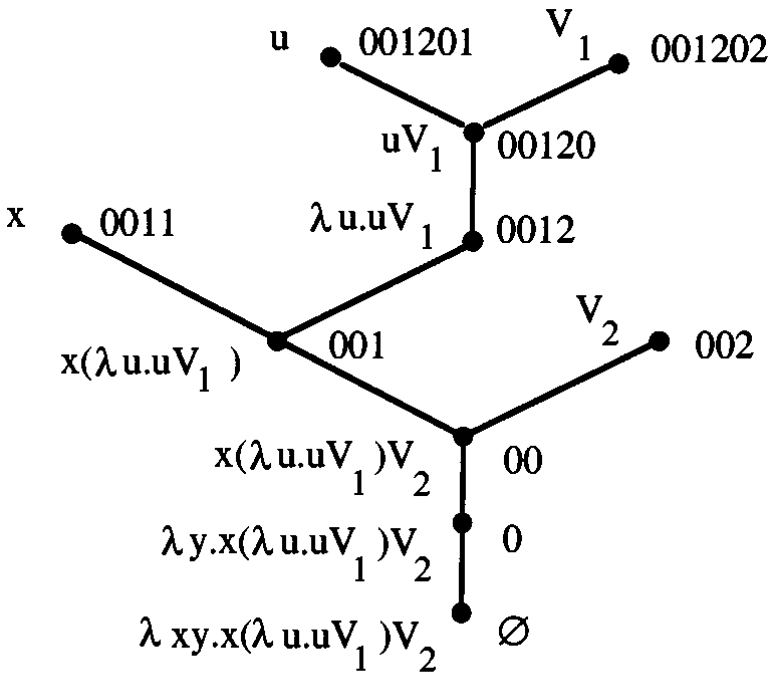
\includegraphics[width=7cm]{fig4.png}
    \caption{Construction Tree for $\lambda xy.x(\lambda u.uV_1)V_2$.
    Figure obtained from \cite{hindley}.}
    \label{fig_construction}
\end{figure}
    
\end{frame}

\subsection{The Foundation for 8F}
\begin{frame}{Subarguments}
\begin{definition}[8E2 in Hindley's]
A subargument of a typed or untyped nf-scheme $X$ is a component that is an argument of $X$ or an argument of a proper component of $X$.
\end{definition}
\end{frame}

\begin{frame}{Lemma 8E2.1}
\begin{lemma}[8E2.1 in Hindley's]
A component \underbar{$Y$} of a typed or untyped nf-scheme $X$ is a subargument iff 
its position is not $\emptyset$ and the last symbol in its position is 2. 
\end{lemma}

\begin{proof}
\pfsketch \ 
By induction on $|X|$. One can, for instance, consider the subarguments in the tree of Figure \ref{fig_construction}.
\end{proof}
\end{frame}

\begin{frame}{Remarks about Subarguments}
\begin{remark}[8E2.2(i) in Hindley's]
All occurrences of meta-variables in a composite nf-scheme are subarguments.
\begin{proof}
\pf \ By restriction 8C1(iii) in the definition of nf-scheme. 
\end{proof}
\end{remark}

\medskip

\begin{remark}[8E2.2(ii) in Hindley's]
A subargument of a subargument of $X$ is a subargument of $X$.
\begin{proof}
\pf \ By the definition of subargument. 
\end{proof}
\end{remark}
\end{frame}

\begin{frame} {2-length and depth}
\begin{mydef}[8E3 in Hindley's]
The 2-length of a position string $p$ is the number of 2's in $p$. 
\end{mydef} 

\medskip 
\begin{mydef}[8E3 in Hindley's]
The depth in $X$ of a subargument $\underbar{Z}$ of $X$ is the 2-lenght of its position. 
\end{mydef}

\begin{remark}[8E3 in Hindley's]
The depth in $X$ of a subargument $\underbar{Z}$ is the number of right-hand choices made when ``travelling up'' the tree of $X$ from the bottom node to $\underbar{Z}$.  
\end{remark}
\end{frame}

\begin{frame}{Lemma 8E3.1}

\begin{lemma}[8E3.1 in Hindley's]
Let $X$ be a typed or untyped nf-scheme with $Depth(X) \geq 1$, where the $Depth$ of an nf-scheme is defined as in 8A6. Then: 
\begin{enumerate}
\item $Depth(X)$ is the maximum of the depths in $X$ of all subarguments in $X$, 
\item $X$ has at least one subargument whose depth in $X$ is the same as $Depth(X)$, and each such subargument is an atom or abstracted atom. 
\end{enumerate} 
\end{lemma}

\begin{proof}
\pfsketch \ By induction on $|X|$, using 8A6. 
\end{proof} 
\end{frame} 

\begin{frame}{Argument-Branch}
\begin{mydef}[8E4 in Hindley's]
If $Z$ is a subargument of a typed or untyped nf-scheme $X$, the \textbf{argument-branch} from $X$ to $Z$ is the sequence: 

\begin{equation*}
\langle \underbar{Z}_0, \underbar{Z}_1, \ldots, \underbar{Z}_k  \rangle
\end{equation*}

such that $\underbar{Z}_0 \equiv \underbar{X}$, $\underbar{Z}_k \equiv \underbar{Z}$ and for each $i = 1, \ldots, k$, we have   $\underbar{Z}_i$ is an argument of $\underbar{Z}_{i-1}$.

\medskip

It is \textbf{unextendable} iff $\underbar{$Z$}$ is an atom or abstracted atom. 

\medskip 

Its \textbf{length} is $k$ (not $k+1$). 
\end{mydef}
    
\end{frame}

\begin{frame}{Lemma 8E4.1}
\begin{lemma}[8E4.1 in Hindley's]
For any typed or untyped nf-scheme $X$:
\begin{enumerate}
\item The depth in $X$ of a subargument $\underbar{$Z$}$ is the same as the length of the argument-branch from $\underbar{X}$ to $\underbar{Z}$, 
\item $Depth(X)$ is the maximum of the lengths of all argument-branches in $X$. 
\end{enumerate}
\end{lemma}

\begin{proof}
\pfsketch \ For (1) use induction on $|X|$, for (2) use 8E3.1.  
\end{proof}
\end{frame}

\begin{frame}{IA, CA}
\begin{mydef}[8E5 in Hindley's]
Let $\underbar{$Z$}$ be a subargument of a typed or untyped nf-scheme $X$, for instance: 

\begin{equation*} 
Z \equiv \lambda x_1 \ldots x_m.y Z_1 \ldots Z_n \tag{$m \ge 0, n \ge 0$}
\end{equation*}

The \textbf{Initial Abstractors sequence IA(Z)} is the (possibly empty) sequence: 
\begin{equation*}
    IA(Z) = \langle x_1, \ldots, x_m \rangle
\end{equation*}

The \textbf{Covering Abstractors sequence CA(\underline{Z}, X)} is defined as: 
\begin{equation*}
    CA(\underbar{Z}, X) = \langle z_1, \ldots, z_q \rangle, 
\end{equation*}

where $\underline{\lambda z}_1$, \ldots, $\underline{\lambda z}_q$ are the abstractors in $X$ whose scopes contain \underbar{$Z$}, written in the order they occur in $X$ from left to right. Also, define: 
\begin{align*}
    Length(IA(Z)) &= m, \\
    Length(CA(\underbar{Z}, X)) &= q.
\end{align*}

\end{mydef}
\end{frame} 

\begin{frame}{IA, CA}
\begin{remark}[8E5.1 in Hindley's]
\begin{enumerate}
    \item If $X$ has no bound-variable clashes, the members of $IA(Z)$ are distinct and so are those of $CA(\underbar{Z}, X)$. 
    \item $IA(Z)$ and $CA(\underbar{Z}, X)$ are sequences of variables, not components. 
    \item For typed nf-schemes each variable in $IA(Z)$ or $CA(\underbar{Z}, X)$ is typed. 
    \item If the argument-branch from \underbar{$X$} to \underbar{$Z$} is $\langle \underbar{Z}_0, \ldots, \underbar{Z}_k \rangle$ ($k \geq 1)$, then: 
    \begin{equation*}
        CA(\underbar{Z}, X) = IA(Z_0) * \ldots * IA(Z_{k-1})
    \end{equation*}
    where ``*'' denotes concatenation of sequences.
\end{enumerate}
\end{remark} 
\end{frame}

\begin{frame}{Warning}
The remaining part of this section applies only for typed nf-schemes. 
\end{frame}

\begin{frame}{IAT}
\begin{mydef}[IAT]
Let \underbar{$Z^\sigma$} be a subargument of a typed nf-scheme $X^\tau$, say: 
\begin{equation*}
    Z^{\sigma} \equiv \lambda x_{1}^{\sigma_1}
    \ldots x_{m}^{\sigma_m}.y Z_1 \ldots Z_n     \tag{$m \geq 0, n \geq 0$}
\end{equation*}

The \textbf{Initial Abstractors' Types Sequence ($IAT(Z^\sigma)$)} is defined as: 
\begin{equation*}
    IAT(Z^{\sigma}) = \langle \sigma_1, \ldots, \sigma_m \rangle; 
\end{equation*}

And we also define:
\begin{equation*}
    Length(IAT(Z^\sigma)) = m
\end{equation*} 
\end{mydef}
\end{frame}

\begin{frame}{Premises}
    If $\rho \equiv \rho_1 \rightarrow \ldots \rightarrow \rho_m \rightarrow a$, we call $\rho_1, \ldots, \rho_m$ the premises of $\rho$ and we call $a$ the tail of $\rho$.
\end{frame}

\begin{frame}{Positions in a Term}
Consider $\tau \equiv (a \rightarrow b \rightarrow c) \rightarrow (a \rightarrow b) \rightarrow a \rightarrow c$. 
\begin{figure}
    \centering
    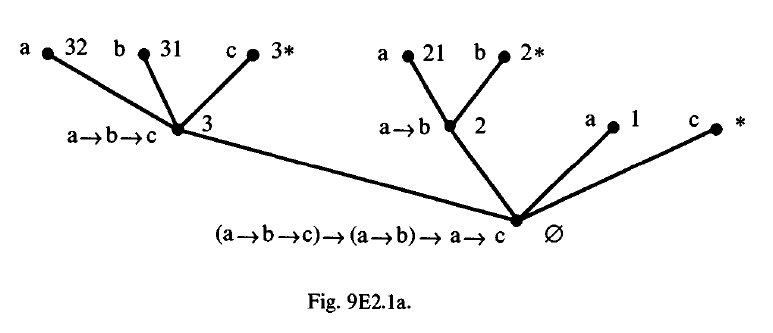
\includegraphics[width=7cm]{subpremise.png}
    \caption{Positions in the term $\tau \equiv (a \rightarrow b \rightarrow c) \rightarrow (a \rightarrow b) \rightarrow a \rightarrow c$.
    Figure obtained from \cite{hindley}.}
    \label{subpremise1}
\end{figure}
\end{frame}

\begin{frame}{Subpremises}
    A subpremise of $\tau$ is a premise of some component of $\tau$ (possibly of $\tau$ itself).
\end{frame}

\begin{frame}{Subpremises}
    \begin{exa}
    \label{ex_subpremises}
    Let $\tau \equiv (a \rightarrow b \rightarrow c) \rightarrow (a \rightarrow b) \rightarrow a \rightarrow c$ (see Figure \ref{subpremise1}). Let's represent subpremisses as triples ``$\langle \text{term}, \text{position}, \tau  \rangle$''. The six subpremisses of $\tau$ are: 
    \begin{enumerate}
        \item $\langle a, 1, \tau \rangle$,
        \item $\langle a \rightarrow b, 2, \tau \rangle$,
        \item $\langle a \rightarrow b \rightarrow c, 3, \tau \rangle$, 
        \item $\langle a, 21, \tau \rangle$,
        \item $\langle b, 31, \tau \rangle$,
        \item $\langle a, 32, \tau \rangle$. 
    \end{enumerate}
    \end{exa}
\end{frame}

\begin{frame}{Positive Subpremises}
    A subpremise of $\tau$ is positive if and only if its position has even length (the symbol $*$ does not count when computing the length). 
    
    \medskip 
    
    In Example \ref{ex_subpremises} the positive subpremises are: 
    \begin{enumerate}
        \item $\langle a, 21, \tau \rangle$,
        \item $\langle b, 31, \tau \rangle$,
        \item $\langle a, 32, \tau \rangle$.
    \end{enumerate}
    
\end{frame}

\begin{frame}{NSS}
\begin{mydef}
$NSS(\tau)$ is the set of all finite sequences 
$\langle \sigma_1, \ldots, \sigma_n \rangle \ \ (n \geq 1)$ such that: 
\begin{equation}
    \sigma_1 \rightarrow \ldots \rightarrow \sigma_n \rightarrow a
\end{equation} 
is positive in $\tau$. 
\end{mydef}

\begin{remark}
Each member of $NSS(\tau)$ is called a negative subpremise-sequence, because it is a sequence of terms that have occurrences as negative subpremises in $\tau$.  
\end{remark}
\end{frame}

\begin{frame}{NSS}
\begin{exa}
\label{ex_nss}
Let $\tau \equiv (a \rightarrow (b \rightarrow d \rightarrow c) \rightarrow d)\rightarrow (a \rightarrow b \rightarrow c) \rightarrow d \rightarrow d$. 

We have $NSS(\tau) = \{ \langle a \rightarrow (b \rightarrow d \rightarrow c) \rightarrow d, a \rightarrow b \rightarrow c, d \rangle, \langle b, d \rangle \}$.
\end{exa}
\end{frame}

\begin{frame}{NSS}
\begin{proof}
\pf
\step{1}{$NSS(\tau) \supseteq \{ \langle a \rightarrow (b \rightarrow d \rightarrow c) \rightarrow d, a \rightarrow b \rightarrow c, d \rangle, \langle b, d \rangle \}$}
\begin{proof}

\step{1-1}{$\langle a \rightarrow (b \rightarrow d \rightarrow c) \rightarrow d, a \rightarrow b \rightarrow c, d \rangle \in NSS(\tau)$}
\begin{proof}
By definition, since:
\begin{equation*}
(a \rightarrow (b \rightarrow d \rightarrow c) \rightarrow d)\rightarrow (a \rightarrow b \rightarrow c) \rightarrow d \rightarrow d
\end{equation*}
is positive in $\tau$, as it has position $\emptyset$, of even length. 
\end{proof}

\medskip 

\step{1-2}{$\langle b, d \rangle \in NSS(\tau)$}
\begin{proof} 
By definition, since: 
\begin{equation*}
    b \rightarrow d \rightarrow c
\end{equation*}
is positive in $\tau$ as it has position 31, of even length. 
\end{proof} 

\end{proof}

\medskip

\step{2}{$NSS(\tau) \subseteq \{ \langle a \rightarrow (b \rightarrow d \rightarrow c) \rightarrow d, a \rightarrow b \rightarrow c, d \rangle, \langle b, d \rangle \}$}
\begin{proof} 
By checking that no other finite sequence $\langle \sigma_1, \ldots, \sigma_n \rangle$ is such that $\sigma_1 \rightarrow \ldots \rightarrow \sigma_n \rightarrow a$ is positive in $\tau$.  
\end{proof}
\end{proof}
\end{frame}

\begin{frame}{NSS}
\begin{mydef}
The set of all the members of the sequences in $NSS(\tau)$ will be called $\cup NSS(\tau)$
\end{mydef}

\begin{exa}
In Example \ref{ex_nss}, we had: 
\begin{equation*}
    NSS(\tau) = \{ \langle a \rightarrow (b \rightarrow d \rightarrow c) \rightarrow d, a \rightarrow b \rightarrow c, d \rangle, \langle b, d \rangle \}
\end{equation*}
Therefore,
\begin{equation*}
    \cup NSS(\tau) = \{ a \rightarrow (b \rightarrow d \rightarrow c) \rightarrow d, a \rightarrow b \rightarrow c, d, b \}
\end{equation*}

\end{exa}

\end{frame}

\begin{frame}{Lemma 8E7}
\begin{lemma}[8E7 in Hindley's]
If \underbar{$Z^\sigma$} is a subargument of a closed long typed nf-scheme $X^\tau$, then 
\begin{enumerate}
    \item $\sigma$ occurs as a positive subpremise in $\tau$ (as defined in 9E6-8), 
    \item If $\sigma$ is an atom, $IAT(Z^\sigma) = \emptyset$, 
    \item If $\sigma$ is composite, $IAT(Z^\sigma) \in NSS(\tau)$ (defined in 9E9),
    \item $NSS(\sigma) \subseteq NSS(\tau)$.
\end{enumerate}
\end{lemma}
\end{frame}

\begin{frame}[allowframebreaks]{Proof of Lemma 8E7}
\begin{proof} 
\pf
\step{1}{$\sigma$ occurs as a positive subpremise in $\tau$ (as defined in 9E6-8).}
% TODO: comment that in this proof, you can't do induction if you start with an empty context. 
\begin{proof} 
\medskip 
\step{1-1}{If $X^\tau$ is a long member of $\mathbb{TNS}$($\Gamma$) and $\Gamma = \{u_1: \theta_1, \ldots, u_p: \theta_p, V_1: \phi_1, \ldots, V_q: \phi_q\}$ and \underbar{$Z^\sigma$} is a subargument of $X^\tau$, then $\sigma$ occurs as a positive subpremise of $\theta_1 \rightarrow \ldots \rightarrow \theta_p \rightarrow \tau$.}
\begin{proof}
The proof is by induction on $|X^\tau|$.

\medskip 

\step{1-1-1}{\textbf{Basis} If $X^\tau$ is an atom there is no \underbar{$Z^\sigma$} subargument of $X^\tau$, and the conclusion holds vacuously.}

\framebreak

\step{1-1-2}{\textbf{Induction Step}}
\begin{proof}
\step{1-1-2-1}{X has the form: 
\begin{equation*}
    (\lambda x_{1}^{\tau_1} \ldots x_{m}^{\tau_m}.
    (y^{(\rho_1 \rightarrow \ldots \rightarrow \rho_n \rightarrow e)}
    X_{1}^{\rho_{1}} \ldots X_{n}^{\rho_{n}} )^{e}
    )^{\tau_1 \rightarrow \ldots \rightarrow \tau_m \rightarrow e}
\end{equation*} 
where $m, n \geq 0$ and $\tau \equiv \tau_1 \rightarrow \ldots \rightarrow \tau_m \rightarrow e$.}

\medskip 

\step{1-1-2-2}{\casePfkwd \ $Z^{\sigma} \equiv X_{j}^{\rho_j}$.}
\begin{proof} 
\noindent

\step{1-1-2-2-1}{Since $Z^{\sigma} \equiv X_{j}^{\rho_j}$, we have $\sigma \equiv \rho_j$.}

\step{1-1-2-2-2}{Each of $\rho_1, \ldots, \rho_n$ occurs as a positive subpremise of $\theta_1 \rightarrow \ldots \rightarrow \theta_p \rightarrow \tau$.}
\begin{proof}
\noindent
\step{1-1-2-2-2-1}{Using the notation of  \stepref{1-1-2-1} and \stepref{1-1}, we have that either $y \equiv x_i$ for some $i \le m$ or $y \equiv u_i$ for some $i \le p$.}
\step{1-1-2-2-2-2}{\casePfkwd \ $y \equiv x_i$. We have that $\rho_1 \rightarrow \ldots \rightarrow \rho_n \rightarrow e \equiv \tau_i$. Then, the position of each $\rho_j$ in $\theta_1 \rightarrow \ldots \rightarrow \theta_p \rightarrow \tau$ has length 2, making it a positive subpremise.}
\step{1-1-2-2-2-3}{\casePfkwd \ $y \equiv u_i$. Then $\rho_1 \rightarrow \ldots \rightarrow \rho_n \rightarrow e \equiv \theta_i$. Then, the position of each $\rho_j$ has length 2, making it a positive subpremise.}
\end{proof}

\end{proof} 

\medskip 

\step{1-1-2-3}{\casePfkwd \ $Z^{\sigma}$ is a subargument of $X_{j}^{\rho_j}$.}

\begin{proof}
\noindent
\step{1-1-2-3-1}{$X_{j}^{\rho_j}$ is a long member of $\mathbb{TNS}(\{x_{1}:\tau_1, \ldots, x_{m}:\tau_{m} \} \cup \Gamma)$}
\step{1-1-2-3-2}{By IH, $\sigma$ occurs as a positive subpremise of
\begin{equation*}
    \tau_1 \rightarrow \ldots \rightarrow \tau_m \rightarrow \theta_1 \rightarrow \ldots \rightarrow \theta_p \rightarrow \rho_j
\end{equation*}.}
\step{1-1-2-3-3}{\casePfkwd \ $\sigma$ is a positive subpremise of $\rho_j$. Then, by using the result $\langle 5 \rangle 2$ of branch $\langle 4 \rangle 2$ (notice the result holds because we can repeat the argument),  we conclude.}
\step{1-1-2-3-4}{\casePfkwd \ $\sigma$ is a negative subpremise of one of $\tau_1, \ldots, \tau_m, \theta_1, \ldots, \theta_p$. Then $\sigma$ will be a positive subpremise of $\theta_1 \rightarrow \ldots \rightarrow \theta_p \rightarrow \tau$.}
\end{proof}

\end{proof}

\end{proof}

\framebreak

\step{2-2}{Since $X^\tau$ is closed, we can apply \stepref{1-1} with $\Gamma = \emptyset$ and conclude.}

\end{proof}

\framebreak

\step{2}{If $\sigma$ is an atom, $IAT(Z^\sigma) = \emptyset$.}
\begin{proof}
\step{2-1}{$IAT(Z^\sigma)$ coincides with the sequences of all premises of $\sigma$.}
\begin{proof}
\step{2-1-1}{$Z^\sigma$ is long.}
\step{2-1-2}{\letPfkwd \  $IAT(Z^\sigma) = \langle \sigma_1, \ldots, \sigma_m \rangle$. Since $Z^\sigma$ is long, $\sigma \equiv \sigma_1 \rightarrow \ldots \rightarrow \sigma_m \rightarrow e$.}
\end{proof}
\step{2-2}{Since $\sigma$ is an atom, there are no premises. By \stepref{2-1}, $IAT(Z^\sigma) = \emptyset$.}
\end{proof}

\framebreak

\step{3}{If $\sigma$ is composite, $IAT(Z^\sigma) \in NSS(\tau)$ (defined in 9E9)}
\begin{proof}
\step{3-1}{$IAT(Z^\sigma) \in NSS(\sigma)$.}
\begin{proof}
\step{3-1-1}{$Z^\sigma$ is long.}
\step{3-1-1}{\letPfkwd \ $IAT(Z^\sigma) = \langle \sigma_1, \ldots, \sigma_m \rangle$. Then, since $Z^\sigma$ is long, $\sigma \equiv \sigma_1 \rightarrow \ldots \rightarrow \sigma_m \rightarrow e$.}
\step{3-1-3}{By \stepref{3-1-1}, and the definition of $NSS(\sigma)$ (which is only defined for $\sigma$ composite) we conclude.}
\end{proof}
\step{3-2}{$NSS(\sigma) \subseteq NSS(\tau)$.}
\begin{proof}
It will be proved in $\langle 1 \rangle$4.
\end{proof}
\end{proof}

\framebreak

\step{4}{$NSS(\sigma) \subseteq NSS(\tau)$.}
\begin{proof}
\step{4-1}{By \stepref{1}, $\sigma$ occurs as a positive subpremise in $\tau$.} 
\step{4-2}{By the technical lemma 9E9.2(iii), since $\sigma$ occurs as a positive subpremise of $\tau$, we have $NSS(\sigma) \subseteq NSS(\tau)$.}
\end{proof}
\end{proof}
\end{frame}

\begin{frame}{Lemma 8E7}
\begin{remark}
Notice that Lemma 8E7 connects $IAT(Z^\sigma)$, which in general depends on the structure of $Z^\sigma$ and hence implicitly on that of $X^\tau$, with $NSS(\tau)$, which depends on $\tau$ and nothing else. 
\end{remark}
\end{frame}


\begin{frame}{Corollary 8E7.1}
\begin{corollary}[8E7.1 in Hindley's]
    If $X^\tau$ is a closed long typed nf-scheme, the type of each meta-variable in $X^\tau$ either occurs as a positive subpremise of $\tau$ or is $\tau$ itself. 
\end{corollary}

\begin{proof}
\step{1}{\casePfkwd \ $X^\tau$ is a composite nf-scheme.}
\begin{proof}
\step{1-1}{\letPfkwd \ $Z^\sigma$ be an arbitrary metavariable in $X^\tau$.}
\step{2-1}{An occurrence of $Z^\sigma$ in $X^\tau$ is a subargument.}
\step{3-1}{Then, by Lemma 8E7, $\sigma$ occurs as a positive subpremise of $\tau$.}
\end{proof}

\medskip 

\step{2}{\casePfkwd \ $X^\tau$ is an atomic nf-scheme.}
\begin{proof}
In this case, $X^\tau$ is a meta-variable. 
\end{proof} 
\end{proof}

\end{frame}

\begin{frame}[allowframebreaks]{Corollary 8E7.2}
\begin{corollary}[8E7.2 in Hindley's]
If $X^\tau$ is a closed long typed nf-scheme and \underbar{$Z^\sigma$} is a subargument of $X^\tau$ or \underbar{$Z^\sigma$} $\equiv$ \underbar{$X^\tau$}, then: 
\begin{enumerate}
    \item Length($IA(Z^\sigma)$) = Length($IAT(Z^\sigma)$) $\leq |\tau| - 1$, 
    \item Length($CA($\underbar{$Z^{\sigma}$}, $X^\tau$)) $\le (|\tau|-1) \times$ Depth($X^\tau$), 
    \item If $\underline{\lambda v}_{1}^{\rho_1}$, $\ldots$, $\underline{\lambda v}_{r}^{\rho_r}$ are all abstractors in $X^\tau$ (not just the initial ones), then $\{\rho_1, \ldots, \rho_r \}$ has $\le |\tau|-1$ distinct members.  
\end{enumerate}
\end{corollary}
\end{frame}

\begin{frame}[allowframebreaks]{Corollary 8E7.2}
\begin{proof}
\step{1}{Length($IA(Z^\sigma)$) = Length($IAT(Z^\sigma)$) $\leq |\tau| - 1$}

\begin{proof}

\medskip 

\step{1-1}{\letPfkwd \  $Z^\sigma \equiv \lambda x_{1}^{\sigma_1} \ldots x_{m}^{\sigma_m}.
y Z_{1}\ldots Z_{n}$}

\medskip 

\step{1-2}{Length($IA(Z^\sigma)$) = Length($IAT(Z^\sigma)$) $= m$.}
\begin{proof}
By definition, $IA(Z^\sigma) = \langle x_1, \ldots, x_m \rangle$ and $IAT(Z^\sigma) = \langle \sigma_1, \ldots \sigma_m \rangle$. 
\end{proof}

\medskip 

\step{1-3}{Length($IAT(Z^\sigma)$) $\leq |\tau| - 1$}
\begin{proof}
\step{1-3-1}{\casePfkwd \ $\sigma$ is atomic. Then, $IAT(Z^\sigma) = \emptyset$ by Lemma 8E7(ii). Therefore, Length($IAT(Z^\sigma)$) = 0 and since $|\tau| \geq 1$ the inequality holds.}

\step{1-3-2}{\casePfkwd \ $\sigma$ is composite.}
\begin{proof}
\step{1-3-2-1}{$IAT(Z^\sigma) \in NSS(\tau)$}
\begin{proof}
By Lemma 8E7(iii). 
\end{proof}
\step{1-3-2-2}{$IAT(Z^\sigma) = \langle \sigma_1, \ldots, \sigma_m \rangle$.}
\begin{proof}
By definition. 
\end{proof}
\step{1-3-2-3}{If $\langle \sigma_1, \ldots, \sigma_m \rangle \in NSS(\tau)$ then $m \leq |\tau|-1$.}
\begin{proof}
By Lemma 9E9.3(iv)
\end{proof}
\end{proof}
\end{proof} 
\end{proof}

\framebreak 

\step{2}{Length($CA($\underbar{$Z^{\sigma}$}, $X^\tau$)) $\le (|\tau|-1) \times$ Depth($X^\tau$)}
\begin{proof}
\medskip 

\step{2-1}{\casePfkwd \ \underbar{Z} $\equiv$ \underbar{X}.}
\begin{proof}
Since no abstractor in $X$ has scope containing \underbar{Z} $\equiv$ \underbar{X}, Length($CA($\underbar{$Z^{\sigma}$}, $X^\tau$)) = 0. 
\end{proof}

\medskip 

\step{2-2}{\casePfkwd \ \underbar{Z} $\not\equiv$ \underbar{X}.}
\begin{proof}

\medskip 

\step{2-2-1}{\letPfkwd \  $\langle$ \underbar{$Z_0$}, $\ldots$, \underbar{$Z_k$} $\rangle$, with $k \geq 1$ be the argument-branch from \underbar{X} to \underbar{Z}.}

\medskip 

\step{2-2-2}{Length(CA(\underbar{Z}, X)) = Length(IA($Z_0$))+ \ldots + Length(IA($Z_{k-1}$)).}
\begin{proof} 
By 8E5.1, remembering that in an nf-scheme there are no bound-variable clashes.
\end{proof} 

\medskip 

\step{2-2-3}{Length(IA($Z_0$))+ \ldots + Length(IA($Z_{k-1}$)) $\le k(|\tau| - 1)$}
\begin{proof}
By Step \stepref{1} we have Length(IA($Z_i$)) $\le (|\tau| - 1)$.  
\end{proof}

\medskip 

\step{2-2-4}{$k(|\tau|-1) \le (|\tau|-1) \times Depth(X)$}
\begin{proof}
By 8E4.1(ii), $Depth(X)$ is greater or equal than the length of the argument-branch from X to Z, which is $k$. 
\end{proof}
    
\end{proof}
\end{proof}

\framebreak 

\step{3}{If $\underline{\lambda v}_{1}^{\rho_1}$, $\ldots$, $\underline{\lambda v}_{r}^{\rho_r}$ are all abstractors in $X^\tau$ (not just the initial ones), then $\{\rho_1, \ldots, \rho_r \}$ has $\le |\tau|-1$ distinct members.}

\medskip 

\begin{proof}
\step{3-1}{$\rho_i \in \cup NSS(\tau)$.}
\begin{proof}
\medskip 

\step{3-1-1}{Each $\rho_i$ is in $IAT(X^\tau)$ or in $IAT(Y^\theta)$ for some subargument $Y^\theta$ of $X^\tau$.}

\medskip 

\step{3-1-2}{\casePfkwd \ $\rho_i \in IAT(X^\tau)$. By the definition of $IAT(X^\tau)$ and of $\cup NSS(\tau)$ we get that $\rho_i \in \cup NSS(\tau)$.}

\medskip 

\step{3-1-3}{\casePfkwd \ $\rho_i \in IAT(Y^\theta)$. By Lemma 8E7(iii) we get that $\rho_i \in \cup NSS(\tau)$.}
\end{proof}

\medskip 

\step{3-2}{$|\cup NSS(\tau)| \leq |\tau| - 1$}
\begin{proof}
By Lemma 9E9.3
\end{proof}
\end{proof}

\end{proof}

\end{frame}



